\newcommand{\figureSPIShiftRegisterConnections}[1]{
  \def\lang{\detokenize{#1}}
  \def\langRu{\detokenize{ru}}
  \def\langEn{\detokenize{en}}
  \def\figureCaption{XXX: No translation.}
  \ifx \lang\langRu
  \def\figureCaption{
    Подключение контроллера к последовательно-параллельному сдвиговому регистру
    по шине SPI.
  }
  \fi
  \ifx \lang\langEn
  \def\figureCaption{
    Connection of a controller to a \gls{SIPO} shift register by the SPI bus.
  }
  \fi
  \begin{figure}[ht]
    \centering
    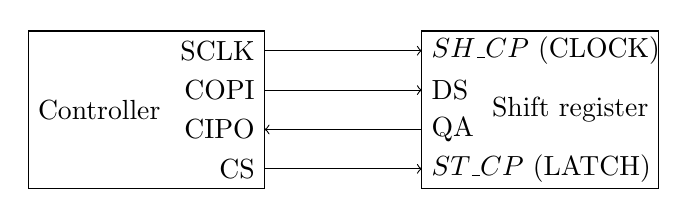
\begin{tikzpicture}
      %% Rectangles.
      \draw[] (0, 0) rectangle (3, 2);
      \draw[] (5, 0) rectangle (8, 2);
      %% Arrows.
      \draw[->] (3, 1.75) -- (5, 1.75);
      \draw[->] (3, 1.25) -- (5, 1.25);
      \draw[<-] (3, 0.75) -- (5, 0.75);
      \draw[->] (3, 0.25) -- (5, 0.25);
      %% Text.
      \node[anchor=west] at (0, 1) {Controller};
      \node[anchor=east] at (3, 1.75) {SCLK};
      \node[anchor=east] at (3, 1.25) {COPI};
      \node[anchor=east] at (3, 0.75) {CIPO};
      \node[anchor=east] at (3, 0.25) {CS};
      \node[anchor=east] at (8, 1) {Shift register};
      \node[anchor=west] at (5, 1.75) {$SH\_CP$ (CLOCK)};
      \node[anchor=west] at (5, 1.25) {DS};
      \node[anchor=west] at (5, 0.75) {QA};
      \node[anchor=west] at (5, 0.25) {$ST\_CP$ (LATCH)};
    \end{tikzpicture}
    \caption{\figureCaption}
    \label{fig:spi-sipo-register}
  \end{figure}
}
